\clearpage
\section{Annex}
\begin{figure}[ht!]
    \centering
        \begin{subfigure}[b]{0.40\textwidth}
            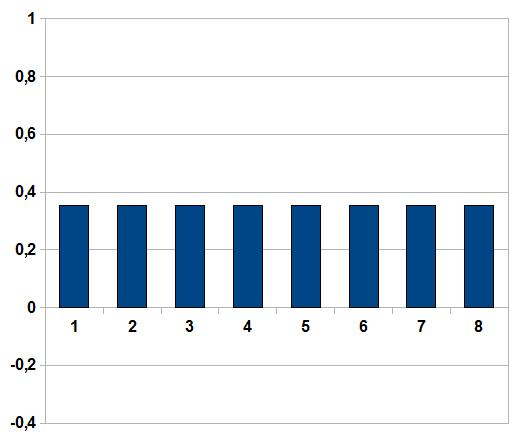
\includegraphics[width=\textwidth]{Grover-EtatInitial.jpg}
            \caption{\footnotesize Initial state $|\psi_{(0)}\rangle$}
            \label{fig2:first}
        \end{subfigure}
        \hspace{1cm}
        \begin{subfigure}[b]{0.40\textwidth}
            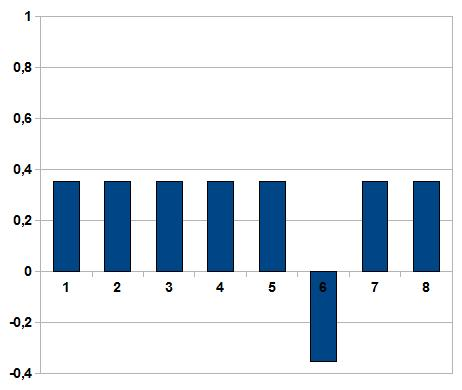
\includegraphics[width=\textwidth]{Grover-PassageParBoiteNoire.jpg}
            \caption{\footnotesize Passage through the oracle $U_{\omega}$}
            \label{fig2:second}
        \end{subfigure}
        \\
        \begin{subfigure}[b]{0.40\textwidth}
            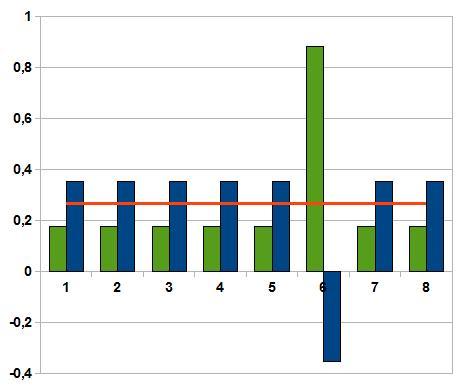
\includegraphics[width=\textwidth]{Grover-MiroirMoyenne.jpg}
            \caption{\footnotesize Passage through the diffusion operator $U_{\psi}$}\footnotemark
            \label{fig2:third}
        \end{subfigure}
        \hspace{1cm}
        \begin{subfigure}[b]{0.40\textwidth}
            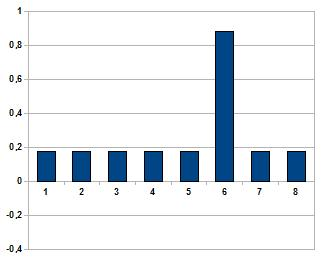
\includegraphics[width=\textwidth]{Grover-Amplification.jpg}
            \caption{\footnotesize Resulting state $|\psi_{(1)}\rangle$ after the first iteration}
            \label{fig2:fourth}
        \end{subfigure}
        \\
        \begin{subfigure}[b]{0.40\textwidth}
            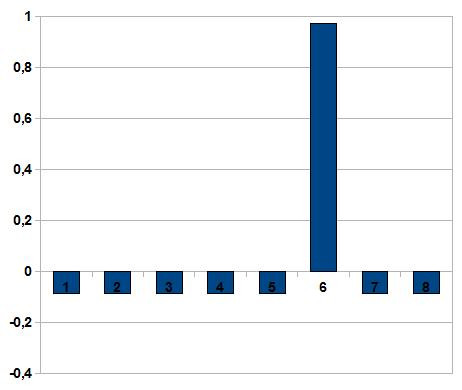
\includegraphics[width=\textwidth]{Grover-EtatFinal.jpg}
            \caption{\footnotesize Final state $|\psi_{(r)}\rangle$  maximizing the amplitude of $|\omega\rangle$ for $\omega=6$}
            \label{fig2:fifth}
        \end{subfigure}

    \caption{\small  Grover's algorithm for $\omega=6 \in [\![1,8]\!]$;  evolution of state vector amplitudes.}
    \label{fig2:subfigures}
\end{figure}

\footnotetext{The red line corresponds to the amplitude of $U_{\omega}|\psi_{(0)}\rangle$, and the blue histogram corresponds to the amplitudes of each of its components. The green histogram represents the amplitudes of the components of $|\psi_{(1)}\rangle = U_{\psi}U_{\omega}|\psi_{(0)}\rangle$, showing that it is a reflection of the blue histogram about the red line.}
